\providecommand{\main}{../../main}
\documentclass[../../main.tex]{subfiles}

\makeglossaries
\loadglsentries{glossary/glossary}

\begin{document}

\chapter{The CMS experiment}
\label{sec:CMS_exp}

Searching for exotic particles never observed before implies a need for an enormous amount of energy in the processes involved in their creation. In fact, if we want to study something never observed before at the scales of energy normally reached, it is highly unlikely we will find something new and interesting. This is the reason for which the Large Hadron Collider, briefly LHC, was designed and built. LHC is actually the world’s largest and most powerful particle accelerator. Its project was conceived in 1976 when the European particle physics community began to discuss building a \acrfull{lep} collider at \acrshort{cern}, and it was realized between 1998 and 2008. It required a collaboration of over 10000 scientists and hundreds of universities and laboratories, as well as more than 100 countries. It first started up on 10 September 2008, and remains the latest addition to CERN’s accelerator complex.

\begin{figure}[h]
    \centering
    \includegraphics[width=0.9\textwidth]{sections/01/Images/Cern_acc_complex.png}
    \caption{CERN accelerator complex, image taken from \cite{LHC-Acc}.}
    \label{fig:CERN_ACC}
\end{figure}  
    
The LHC consists of a ring 27-kilometers long of superconducting magnets with a number of accelerating structures to boost the energy of the particles along the way. Inside the accelerator, two high-energy particle beams travel at relativistic speed, close to the speed of light c. Before they are made to collide, they both are accelerated to a energy of the order of TeV. The two beams travel in opposite directions in separate beam pipes, which are fundamentally two tubes kept at ultrahigh vacuum. They are guided around the accelerator ring by a strong magnetic field mainteined by superconducting electromagnets, built from coils of special electric cable that operates in a superconductive state. It is of primary importance to conduct electricity with the lowest resistance, therefore loss of energy, possible. Such technique requires cooling the magnets to a temperature close to 0 K, which is even colder than the outer space. In order to get those temperatures, much of the accelerator is connected to a distribution system of liquid helium and the cooling phase takes a long time. Thousands of magnets of different varieties and sizes are exploited to direct the beams around the accelerator. In total, there are\footnote{Technical details taken from the official CERN website\cite{LHC}} :
\begin{itemize}
    \item 1232 dipole magnets whose length is 15 metres and their purpose is bending the beams;
    \item 392 quadrupole magnets, each 5-7 metres long, which focus the beams, thanks to their properties
    of magnetic lens;
\end{itemize}
Just prior to collision, another type of magnet is used to ‘squeeze’ the particles closer together to increase the chances of collisions. In fact, the particles can be imagined as very tiny objects, so it is clear that the task of making them collide must be thought with such precision. The beams inside LHC are made to collide at four locations around the accelerator ring, corresponding to the positions of four particle detectors: CMS, ATLAS, ALICE and LHCb.  
    
A brief introduction of the main collision points in given below.
\begin{itemize}
    \item \textbf{\acrshort{atlas}}:A Toroidal LHC ApparatuS, general purpose detector located in Meyrin, Switzerland. It is the largest detector in LHC, built with same purpose of the other general purpose detector CMS.
    \item \textbf{\acrshort{cms}}:Compact Muon Solenoid, general purpose detector located in Cessy, France. As its name suggest it is quite dense, leaving little empty space between its detectors.
    \item \textbf{\acrshort{lhcb}}:LHC beauty, specialized in the so-called b-Physics, it is located near Fernay-Voltaire, France. Designed primarily to measure the parameters of CP violation in the b-hadrons interactions.
    \item \textbf{\acrshort{alice}}:A Large Ion Collider Experiment, detector specialized in Pb-Pb collisions, located in Saint-Genis-Pouilly, France. Characterized by large event size, with lower trigger rate compared to other experiments.
\end{itemize}

\begin{figure}[h]
    \centering
    \includegraphics[width=0.9\textwidth]{sections/02/Images/cms_160312_02.png}
    \caption{The CMS detector is shaped like a cylindrical onion, with several concentric layers of components. Taken from Ref. \cite{CMS}.}
    \label{fig:CMS_det}
\end{figure}

\section{CMS detector}

The CMS detector is located in Cessy (France) at the intersection point 5 of the LHC. A diagram of the Run-1 CMS detector is displayed in Fig. \ref{fig:CMS_old}. CMS is a quasi-hermetic, general-purpose detector that covers the entire azimuthal angle φ and pseudo-rapidity η between $-5.2$ and $5.2$. The large solid angle coverage and variety of complementary subdetectors enable CMS to measure a broad range of physics phenomena. Subdetectors are installed in a layered structure where each layer serves a specific function. The layers can be summarised from the inside out as:
\begin{itemize}
    \item \textbf{Silicon tracker}: identifies interaction vertices, reconstructs the tracks of charged particles, whose bending radius due to the magnetic field is used to obtain the associated particle’s charge and momentum.
    \item \textbf{\acrfull{ecal}}: measures the energy of photons and electrons, and contributes to the reconstruction of the charged hadrons.
    \item \textbf{\acrfull{hcal}}: measures the energy of charged and neutral hadrons.
    \item \textbf{Superconducting solenoid}: produces a 3.8 T magnetic field in the inner part and a 2 T field in the flux return yoke that is used to bend the tracks of charged particles.
    \item \textbf{Muon chambers}: measures the tracks of muons and their momentum in synergy with the silicon tracker.
\end{itemize}

\begin{figure}[h]
    \centering
    \includegraphics[width=0.7\textwidth]{sections/02/Images/CMS_OLD.png}
    \caption{Diagram of the Run-1 CMS detector.}
    \label{fig:CMS_old}
\end{figure}

CMS will be upgraded in view of the HL-LHC upgrade. The upgraded detector is referred to as Phase-2 CMS, in contrast to Phase-1 CMS, which is the detector used after the Run-2 of LHC. Phase-2 CMS will retain the same layered structure. Many subdetectors will be replaced or upgraded in order to maintain the same reconstruction performance under more demanding pile-up conditions. Most of the electronics front-end and back-end will be upgraded to cope with the increased data rates. In the following sections, both Phase-1 and Phase-2 versions of each CMS layer will be briefly presented.
        
\section{Silicon tracker}
\label{sec:Si-track}
The silicon tracker \cite{Si-track} is used to obtain the tracks of charged particles and infer their momentum and charge. It also identifies the primary vertex. The Phase-1 silicon tracker provides good performance up to $|\eta| =$ 2.5. The tracker is composed of two different subdetectors of finer granularity as they approach the interaction point in order to maintain the same track reconstruction performance as the particle density increases. The inner subdetector employs pixel detectors; each pixel is 100 $\times$ 150 $\mu m$ 2 big in the $\varphi \times \eta$ directions. Micro strip silicon detectors surround the pixel detectors; the size of each strip increases with distance from the beam pipe.  
The Phase-2 upgrade \cite{Si-track-up} of the tracker will be able to build tracks of particles up $| \eta| =$ 4.  

The inner sector of the tracker will be equipped with silicon pixels 25 $\times$ 100 $\mu m^2$  or 50 × 50 $\mu m^2$ big in $\varphi \times \eta$ . The outer tracker will be composed of silicon strip pairs, and will be able to provide track stubs built from hit doublets to the trigger. In order to reduce data rates, only stubs above a specific $p_T$ threshold will be sent out. The selection is performed via modules called $p_T$ modules.  
A schematic of how the filtering is applied is shown in Fig. \ref{fig:Si-stubs} for each hit, an acceptance window, marked in green in the picture, is created in the second layer; stubs whose second hit is found within the window are considered to have $p_T$ higher than the threshold and sent out. The magnetic field bends the tracks of charged particles; a narrow window corresponds to a higher $p_T$ threshold. A $p_t$ threshold of 2 GeV is sufficient to reduce data rates by an order of magnitude and fit in the bandwidth limits of the system.

\begin{figure}[h]
    \centering
    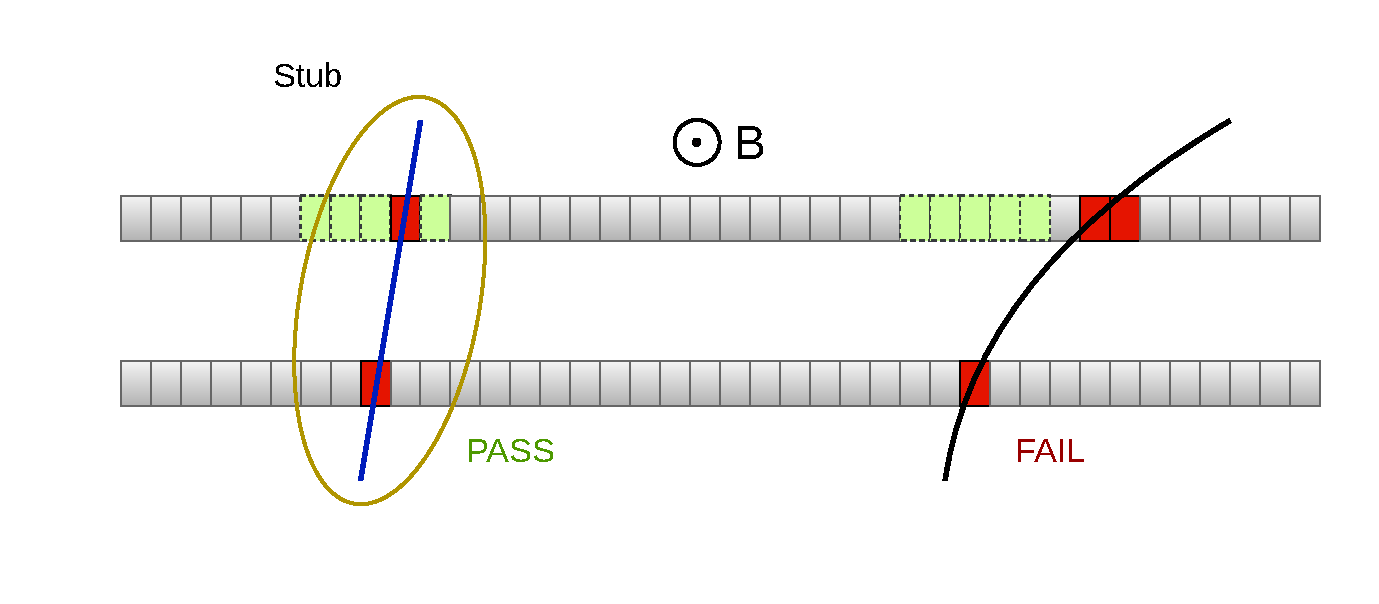
\includegraphics[width=0.9\textwidth]{sections/02/Images/STUB_sitrack.pdf}
    \caption{Illustration of a stub selection based on the $p_t$ value.}
    \label{fig:Si-stubs}
\end{figure}

\section{Electromagnetic and hadron calorimeters}
\sectionmark{Calorimeters}
\label{sec:Calo}

The calorimeters provide an energy measurement of photons, electrons, and charged and neutral hadrons up to $|\eta| = 5$. The barrel, endcap, and forward calorimeter respectively cover the $0 < | \eta | < 1.479$, $1.479 < | \eta | < 3$, $3 < | \eta | < 5$ ranges.  
The barrel and endcap ECAL \cite{ECAL} are equipped with scintillating PbWO 4 crystals of size $0.0174 \times 0.0174$ in $\eta \times \varphi$. Crystals in PbWO 4 were chosen as an active material for their radiation resistance, density ($8.28 g/cm^3$ ), radiation length ($X_0 = 0.89 cm$), and Molière radius ($2.2 cm$). These properties altogether ensure that ECAL is able to contain and measure an electromagnetic shower in a confined space. In addition this material produces around 80\% of the scintillation photons within $25 ns$, providing good time resolution.  

The barrel and endcap HCAL \cite{HCAL} is a sampling calorimeter composed of alternating layers of plastic scintillators and brass, which was chosen as an absorber material due to its non-magnetic
properties. The forward hadron calorimeter (HF) uses quartz fibers and steel absorbers to measure the energy of hadrons via the Cherenkov effect.
The endcap calorimeter will have absorbed a significant amount of radiation by the start of HL-LHC operations and will be replaced by the \acrfull{hgcal} \cite{HGCAL} in the Phase-2 upgrade. HGCAL is a sampling calorimeter with a fine segmentation in both longitudinal and transverse direction, enabling accurate 3D positioning of energy deposits. A
cross section of the upgraded endcap calorimeters is displayed in Fig. \ref{fig:Calorimeter}. The subdetector is divided into electromagnetic and hadron sections. The former is composed of 28 absorber layers
in tungsten and copper alternating with silicon as active material; the latter consists of 12 absorbers layers in brass and copper interleaved with silicon sensors in the front section, and
highly-segmented plastic scintillators in the rear section.  

The reconstruction performance of the CMS detector will greatly benefit from the high granularity information. The high-density of the calorimeter will cause showers to be contained in a small region, which is fundamental in order to prevent overlap between energy deposits coming from different objects in the congested environment of the HL-LHC. The longitudinal and transverse
structure of the energy deposits will be used to discriminate between electromagnetic showers, taus, jets and pile-up. 

\begin{figure}[h]
    \centering
    \includegraphics[width=0.75\textwidth]{sections/02/Images/Calorimeter_phase1.png}
    \caption{Longitudinal cross section of HGCAL. The electromagnetic section is labelled with CE-E, the hadron section with CE-H. Plastic scintillator are colored in blue, silicon detector in green.}
    \label{fig:Calorimeter}
\end{figure}

\section{Muon chambers}
\label{sec:Moun_chamb}

The muon chambers \cite{Muon-cham} employ gaseous detectors to reconstruct tracks of muons exiting the inner part of the detector. Muons are minimum ionising particles that do not get stopped by the detector. Therefore, their momentum is obtained from the curvature of the track left in the tracker and the muon chambers. A magnetic field strong enough to produce a measurable effect on tracks outside the solenoid is ensured by a iron yoke, in which the muon chambers are located.
The yoke also serves the purpose of containing the magnetic field. The barrel muon chambers, covering up to $| \eta | = 1.1$, employ \acrfull{dt} and \acrfull{rpc}. The endcap muon chambers cover the $1.4 < | \etaη | < 2.4$ range and consist of RPCs and \acrfull{csc}.  

Three main upgrades to the muon detectors are expected for the Phase-2 of the experiment \cite{Muon-up}. The existing muon detectors will be upgraded for longevity. \acrfull{gem} detectors will be added in the endcap region for redundancy and to improve the track reconstruction performance. The coverage of the endcap muon detector will be extended up to $\eta \approx 3$.

\section{Level-1 Trigger}
\label{sec:L1T}

The level-1 trigger (L1T) of the CMS experiment will be presented in this section giving an overview of the entire architecture of the trigger system. Firstly, the L1T system used during in the
Phase-1 of the CMS experiment is introduced, then the Phase-2 upgrade of the system will be described, with particular attention to the global trigger implementation, is discussed.  

\begin{figure}[h]
    \centering
    \includegraphics[width=0.6\textwidth]{sections/02/Images/L1T_scheme.png}
    \caption{Diagram of the CMS trigger systems. Taken from Ref. \cite{L1T}}
    \label{fig:L1T_diagram}
\end{figure}

For each bunch crossing, signals are collected by the detector, these data are digitised and stored on front-end pipelines. A subset is processed to produce \acrfull{tps}. TPs are used to build a coarse granularity version of the event that requires less bandwidth and can be sent every bunch crossing to the level-1 trigger. Within a
few $\mu s$ the L1T analyses the TPs within the electronic boards, and issues an accept or reject signal (Level-1 accept, L1A) to the front end buffers. The decision on whether to accept or reject an event is based on a \texit{trigger menu}, i.e. a set of algorithms that define the criteria for which an event is considered interesting.  

An accept signal causes the front end buffer to send the full-event data to the event builder network. The event builder network collects data from all the detector data sources and combines them together to form a single event entity that is sent to the CMS computing services. Here, a \acrfull{hlt} runs offline reconstruction algorithms on a computing cluster. A set of
progressive filters is run in order to further select events in the time scale of a second on average.
Finally, events accepted by the HLT are sent to the CERN computing centre and stored for offline analysis. A diagram of CMS trigger system is shown in Fig. \ref{fig:L1T_diagram}, it is possible to spot the two trigger levels namely the L1 and the HLT, computation is done in custom hardware (FPGA) and commercial hardware (CPU/GPU) respectively.

\subsection{Phase-1 level-1 trigger}
\label{Phase-1_l1T}

The Phase-1 level-1 trigger was commissioned in 2015 and 2016, the upgrade was necessary the in order to maintain the Run-1 physics acceptance at the increased luminosity and rates of
Run-2 \cite{L1T-1up}. The system consists of around 100 hardware boards that process around 5 Tb/s of data. This information is used to reduce the detector readout rate from 40 MHz to a maximum of
100 kHz. The system must complete processing of an event within $3.8 \mu s$, determined by the size of the front end buffer, and be ready to process new data every $25 ns$.


\begin{figure}[h]
    \centering
    \includegraphics[width=0.77\textwidth]{sections/02/Images/Phase-1_l1t.pdf}
    \caption{Diagram of the Phase-1 L1T upgrade. Taken from Ref. \cite{L1T-1up}}
    \label{fig:Phase-1_L1T}
\end{figure}

\subsubsection{Architecture}
\label{Phase-1_l1T_arch}
A diagram of the architecture of the Phase-1 L1T is displayed in Fig. \ref{fig:Phase-1_L1T}. The system has two separate branches, one processing inputs from the muon systems and one from the calorimeters.  



The muon trigger is organised in three different subsystems, each one processing muon hits in a specific $\eta$ range. The barrel muon track finder (\acrshort{bmtf}) find tracks in the $|\eta| < 0.8$ region of the detector, where muons only hit the DTs and RPCs in the barrel. The overlap muon track finder (\acrshort{omtf}) processes data in the $0.8 < |\eta | < 1.25$ region, which corresponds to the overlap between the barrel and the endcap muon detectors. The endcap muon track finder (\acrshort{emtf}) reconstructs muon tracks in the $| \eta | > 1.25$ range, corresponding to the area uniquely occupied by the endcap muon detectors. Muon tracks are found by running pattern matching algorithms. A new algorithm, based on a Kalman filter \cite{Muon_kalman}, will be deployed in the BMTF for Run-3 of CMS, improving the reconstruction performance in the corresponding $\eta$ range.  

The calorimeter trigger receives calorimeter towers, i.e. energy deposited in a group of ECAL crystals and the HCAL tower behind them. The calorimeter trigger is organised in a two-layer structure and uses time-multiplexing to process data from a single event in a single board \cite{TMUX}. An example of time multiplexing is shown in Fig. \ref{fig:TMUX}. In a time multiplexed trigger of period N, a
multiplexing layer sends data from every N-th event to a specific board. In order to constantly process new events, N boards are required. Data from consecutive events are sent to consecutive
boards in a round-robin fashion. In the calorimeter trigger, a time multiplexing period of 9 is used. The first layer serves as a multiplexing stage. The second layer finds calorimeter objects and computes energy sums, e.g. hadron jets and $p^{miss}_T$. The output is sent to a demultiplexing stage which takes care of sorting the objects and transmitting those with highest energy to the global trigger.  

The Global Trigger (GT) runs a set of selection requirements (algorithms in the following) called the \texit{trigger menu}. These algorithms range from single-object $p_T$ thresholds to complex object correlations involving several so-called trigger objects. The GT can run up to 512 selections in parallel. In the final stage, the GT computes a final logical OR on the output of all selection criteria to determine whether to issue a L1A signal.

\begin{figure}[h]
    \centering
    \includegraphics[width=0.67\textwidth]{sections/02/Images/TMUX.png}
    \caption{Example of a time multiplex topology with a \acrshort{tmux} period of 7. Taken from Ref. \cite{TMUX}}
    \label{fig:TMUX}
\end{figure}
%Each Trigger Primitive Generator (TPG in the figure) send its data to the MUX at each LHC clock tick, the MUX will then merge all the partial data and send it to one processor (TMT processor in the figure), the next one will be sent to the subsequent processor in a round-robin scheme. Each processor will receive the packets out of phase of 1 LHC clock tick.

\subsubsection{Global trigger}
\label{Phase-1_l1T_arch}

The Phase-1 upgrade global trigger ($\mu$GT in the following) was necessary due to limitations in the previous Level-1 Trigger and the GT in particular, critical parts are the processing capabilities of the FPGAs and \acrshort{asic}s, as well as the bandwidth constraints in the connections between VME cards. The extensive use of cables causes additional problems, contributing to errors through faults in loose connectors and making maintenance more complicated. The GT upgrade has been designed to be largely independent of a specific hardware solution by using a flexible approach based on existing commercial off-the-shelf components wherever possible. From this point of view, it is simpler to use one common card type for the whole of the Global Trigger to keep maintenance as effortless as possible.

\begin{figure}[h]
    \centering
    \includegraphics[width=0.87\textwidth]{sections/02/Images/P1GT-overview.jpg}
    \caption{Overview of the firmware design of one of the MP7 boards in the $\mu$GT system. Taken from \cite{uGT}.}
    \label{fig:uGT-firmware}
\end{figure}

The whole $\mu$GT system consists in 6 MP7 boards -shown in Fig. \ref{fig:Phase-1_MP7}- equipped with the Virtex-7 FPGA part. Each block is clocked to the LHC frequency, both the algorithm logic and the final decision logic are placed in the same FPGA. The system can run simultaneously up to 512 algorithms distributed on the board pool, the final decision bit is then computed externally combining the output bits from the MP7 boards. The board is built following the \acrshort{utca} standard, hence the name $\mu$GT.

\begin{figure}[h]
    \centering
    \includegraphics[width=0.55\textwidth]{sections/02/Images/MP7_board.jpg}
    \caption{$\mu$TCA standard MP7 board for the Phase-I upgrade.}
    \label{fig:Phase-1_MP7}
\end{figure}

In Fig. \ref{fig:uGT-firmware} is shown the overview of the firmware design of one of the MP7 boards in the $\mu$GT system. Following the data path the signal sees: the input interface, the global trigger logic, the final decision logic and the finally output interface. 


\subsection{Phase-2 level-1 trigger}
\label{Phase-2_l1T}

The Phase-1 L1T is expected to have an accept rate of 1500 kHz if the same trigger menu and algorithms are kept at $\mathcal{L}_{inst} = 5 \times 10^{34} cm^{-2} s^{-1}$ \cite{L1T-2up}. This rate would increase to 4000 kHz at $\mathcal{L}_{inst} = 7 \times 10^{34} cm^{-2} s^{-1}$. It is impossible for the CMS detector to operate and successfully acquire data under these conditions without raising the trigger thresholds and critically compromise its physics reach. The main objective of the Phase-2 upgrade of the L1T is to maintain and potentially expand the physics acceptance of the CMS experiment at the higher luminosity conditions of HL-LHC while remaining within the bandwidth limits of the detector. This is achieved by introducing in L1T a track trigger and high granularity 3D TPs from HGCAL [31], which drastically improve the reconstruction performance of the system. In addition, the readout of the pre-existing subdetectors is upgraded to handle higher L1T accept rates.  


\begin{figure}[h]
    \centering
    \includegraphics[width=0.77\textwidth]{sections/02/Images/Phase-2_l1t.png}
    \caption{Level 1 Trigger block diagrams. Taken from \cite{L1T-2up}}
    \label{fig:Phase-2_L1T}
\end{figure}


The Phase-2 L1T pictured in FIG. \ref{fig:Phase-2_L1T} consists of around 500 boards that analyse an input data rate of 50 Tb/s. The maximum accept rate will be increased to 750 kHz and the maximum latency to $12.5 \mu s$. These improvements enable the Phase-2 L1T to maintain a physics acceptance similar to the Phase-1 system with an accept rate of 260 and 500 kHz at an instantaneous luminosity of $5 \times 10^{34}$ and $ 7 \times 10^{34} cm^{-2} s^{-1}$, respectively \cite{L1T-2up}.  

The Phase-2 L1T is able to compute two types of objects:
\begin{itemize}
    \item \textbf{Standalone objects}: objects reconstructed by using data from a limited set of subdetectors, e.g.
from only the calorimeters;
    \item \textbf{Particle flow objects}: objects found using the particle-flow (PF) algorithm employing the information coming from the different subsystems.
\end{itemize}

The redundancy enables the L1T to be more robust in case of issues. Having track information enables the system to run the \acrfull{puppi} algorithm \cite{PUPPI} for pile-up subtraction, making PF objects extremely resilient to the harsh pile-up conditions of HL-LHC.

\subsubsection{Phase-2 Global trigger}
\label{Phase-2_GT}

The Global Trigger (GT in the following) system is responsible for implementing the so-called trigger menu, i.e. the parallel evaluation of $\sim$1000 trigger algorithms that select a specific event signature. It needs to receive inputs from all upstream trigger systems, buffer data to compensate for different arrival times, de-multiplex data and provide them to the global trigger algorithms, which are all evaluated in parallel. The GT system further provides functionality to pre-scale algorithms and to monitor their rate, both before and after taking into account dead time. Finally, the GT system computes the trigger type based on the trigger algorithms that fired and sends it to the \acrfull{tcds2} \cite{TCDS2}.  

As in Phase-1, the trigger menu is expected to evolve continuously to adapt to the operating conditions provided by the LHC and to new insights gained. The experience from Run-1 and Run-2 shows that more and more complex algorithms tend to be added over time, which are tailored to very specific physics channels. As these algorithms tend to use a lot of resources, the Global Trigger system needs to be scalable. In general, it is desirable that in order to update the trigger menu, only the Global Trigger system needs to be updated, i.e. that all cuts defined in the menu are applied in the Global Trigger.

\begin{figure}[h]
    \centering
    \includegraphics[width=0.89\textwidth]{sections/02/Images/Serenity1v5_combined.png}
    \caption{Top and bottom view of the Serenity board.}
    \label{fig:Phase-2_Serenity}
\end{figure}

It is likely that the firmware of the Global Trigger will need to be regenerated when the menu changes - at least for major changes of the menu (as is the case for the Phase-1 Global Trigger). The software infrastructure to automatically create new firmware based on a description of the menu will be an important deliverable of the Global Trigger project. The firmware is developed to keep frozen the common modules, such as the transceiver and the channel de-multiplexer, and only the algorithm sub-modules will be subjected to the re-generation. From a given new trigger menu, each algorithm will receive a score based on which input it needs and an estimate of its resource requirements, then the tool will try to balance the sum of such score over the SLRs with in the same board and over the board pool.  

The target board of such project is the Serenity\cite{Serenity} shown in FIg. \ref{fig:Phase-2_Serenity}, it is built following the \acrshort{atca} (advanced TCA) standard and it can host up to two daughter cards each of them hosting an Ultracale+ FPGA. On top of that it  also houses a CPU for the communications and a third FPGA (Artix based) to distribute the clock and the controls from the backplane. 

\begin{figure}[h]
    \centering
    \includegraphics[width=0.81\textwidth]{sections/02/Images/GT_TDR.pdf}
    \caption{Architecture of the Phase-2 Global Trigger system.}
    \label{fig:GT-TDR}
\end{figure}

The layout of the complete Global Trigger subsystem is highlighetd in Fig. \ref{fig:GT-TDR}: each algorithm board receives a copy of the same inputs. The number on the top right of the upstream systems indicates the assumed time multiplexing factor of the upstream system. However, other time multiplexing factors can be employed in these systems, as long as the total number of links does not change. Both time axes show the worst-case latency of the GT system, that would be needed, if the upstream system(s) on the critical path had a time-multiplexing factor of 18.

The total latency of the Global Trigger including three optical links (up to TCDS) and deserialization is illustrated in Table \ref{tab:GT-lat}. For input links from upstream systems and the output link to TCDS, in each instance half of the latency of the link is attributed to the GT. The full latency of time de-multiplexing data is attributed to the GT. This brings the total latency of the GT to 1 µs, if the upstream system on the critical path used the highest supported time multiplexing factor of 18.

\begin{table}[h]
    \centering
    \begin{tabular}{|c|c|c|}
        \hline
        \multirow{2}{*}{Item} & \multicolumn{2}{c|}{Latency}   \\
        \cline{2-3}
         & BX & $n s$ \\
         \hline
         Input Link   & 2.5 & 62.5 \\
         Deserializer & $nTMUX$ & $25\times nTMUX$ \\
         Algorithms   & 10 & 250 \\
         Link to Final-OR & 5 & 125 \\
         Final-OR & 2 & 50 \\
         Link to TCDS-2 & 2.5 & 62.5 \\
         \hline
         Total          & $22 + nTMUX$ & $550 + 25\times nTMUX$ \\
         \hline
    \end{tabular}
    \caption{Summary of the expected L1T latency}
    \label{tab:GT-lat}
\end{table}

The baseline for the output to TCDS is a single 10 Gb/s optical fiber transmitting the trigger decision for each bunch crossing. The trigger decision will be encoded as a field of bits, each bit denoting a trigger type. TCDS passes the field of trigger bits on to the sub-detectors. The actual list of trigger types and their meaning or each detector remains to be defined.  
The interface to TCDS also foresees a reverse link that is reserved for future use, such as communicating the dead time or the warning state back, to be used in the trigger throttling.

\clearpage
\subsection{Phase-1 and Phase-2 trigger upgrades}
\label{L1T_summary}

In 2027,2028,2029 during the long shutdown 3, the CMS experiment will be upgraded to retain its physics sensitivity despite the larger background. The level-1 trigger will be completely replaced by a new system equipped with large FPGAs and high-speed optical links running up to 25 Gb/s. The system will receive fine granularity inputs from the calorimeters, and tracks from the tracker and muon chambers. The correlator trigger will be introduced, it is a new \acrshort{l1t} subsystem that will run particle flow algorithms to identify single particles in an event and powerful pile-up subtraction techniques to reject those not produced in the hard interaction vertex.  

A brief table summarizing the main upgrades from Phase-1 to Phase-2 trigger system is shown in \ref{tab:L1T_summary}.


\begin{table}[h]
    \centering
    \begin{tabular}{|c|c|c|}
        \hline
        & Phase-1 & Phase-2 \\
        \hline
        $\left<PU\right>$            & 50    & 200    \\
        Latency [$\mu s$] & $3.8$ & $12.5$ \\
        L1T rate [$kHz$]  & $100$ & $750$  \\
        HLT rate [$kHz$]  & $1$   & $7.5$  \\
        \hline
        \multirow{4}{*}{Subsystems} &  & Calorimeter \\
                                    & Calorimeter & Muon \\
                                    & Muon & Tracker     \\
                                    & & Correlator \\
        \hline
        Board link speed [Gb/s] & 10 & 25 \\
        Board standard & $\mu$TCA  & ATCA \\
        
        
        \hline
    \end{tabular}
    \caption{Summary of the main differences between the two upgrades}
    \label{tab:L1T_summary}
\end{table}



\end{document}